% Created 2019-12-20 Fri 13:02
% Intended LaTeX compiler: pdflatex
\documentclass[12pt]{report}
\usepackage[utf8]{inputenc}
\usepackage[T1]{fontenc}
\usepackage{graphicx}
\usepackage{grffile}
\usepackage{longtable}
\usepackage{wrapfig}
\usepackage{rotating}
\usepackage[normalem]{ulem}
\usepackage{amsmath}
\usepackage{textcomp}
\usepackage{amssymb}
\usepackage{capt-of}
\usepackage{hyperref}
\usepackage{minted}
\usepackage[]{minted}
\usepackage{tcolorbox}
\usepackage{etoolbox}
\def\mytitle{??? Program Code ???}
\BeforeBeginEnvironment{minted}{\begin{tcolorbox}[title=\hfill \mytitle]}%
\AfterEndEnvironment{minted}{\end{tcolorbox}}%
\usepackage{hyperref}
\usepackage{algorithmic}
\makeatletter
\AtBeginEnvironment{minted}{\dontdofcolorbox}
\def\dontdofcolorbox{\renewcommand\fcolorbox[4][]{##4}}
\makeatother
\usepackage[hmargin=25mm,vmargin=25mm]{geometry}
\setlength{\parskip}{1em}
\setlength{\parskip}{1em}
\usepackage[backend=biber,style=alphabetic]{biblatex}
\addbibresource{References.bib}
\usepackage{MyUnicodeSymbols}
\usepackage[dvipsnames]{xcolor} % named colours
\usepackage{color}
\definecolor{darkred}{rgb}{0.3, 0.0, 0.0}
\definecolor{darkgreen}{rgb}{0.0, 0.3, 0.1}
\definecolor{darkblue}{rgb}{0.0, 0.1, 0.3}
\definecolor{darkorange}{rgb}{1.0, 0.55, 0.0}
\definecolor{sienna}{rgb}{0.53, 0.18, 0.09}
\hypersetup{colorlinks,linkcolor=darkblue,citecolor=darkblue,urlcolor=darkgreen}
\author{\href{mailto:dalvescb@mcmaster.ca}{Curtis D'Alves}}
\date{\today}
\title{Analysis of Compiler Heuristics via Stochastic Scheduling and Hyper-Heuristics}
\hypersetup{
 pdfauthor={\href{mailto:dalvescb@mcmaster.ca}{Curtis D'Alves}},
 pdftitle={Analysis of Compiler Heuristics via Stochastic Scheduling and Hyper-Heuristics},
 pdfkeywords={},
 pdfsubject={Thesis proposal for Curtis D'Alves; McMaster University 2019.},
 pdfcreator={Emacs 26.3 (Org mode 9.2.3)}, 
 pdflang={English}}
\begin{document}



\setminted[haskell]{fontsize=\footnotesize}
\setminted[agda]{fontsize=\footnotesize}
\def\labelitemi{$\diamond$}
\def\labelitemii{$\circ$}
\def\labelitemiii{$\star$}

% Level 0                 Level 0
% + Level 1               ⋄ Level 1
%   - Level 2       --->      ∘ Level 2
%     * Level 3                   ⋆ Level 3
%

\begin{center}


\thispagestyle{empty}

{\color{white}{.}}

\vspace{5em}

{\Huge Analysis of Compiler Heuristics via Stochastic Scheduling and Hyper-Heuristics}

\vspace{1em}

{\Large A Thesis Proposal}

\vspace{2em}

Department of Computing and Software

McMaster University

\vspace{2em}
\href{mailto:curtis.dalves@gmail.com}{Curtis D'Alves}

\vspace{2em}
\today

\vfill

\def\mytitle{{\sc Thesis Proposal \hspace{12em} \color{grey}{.} }}
\begin{minted}[]{haskell}
Christopher Anand                                    anandc@mcmaster.ca
Wolfram Kahl                                         kahl@cas.mcmaster.ca
\end{minted}
\end{center}

\begin{abstract}


In compiler optimization, Instruction Scheduling seeks to optimize the order of
a sequence of instructions to maximize throughput while preserving semantics. As
modern architectures become increasing more complex, with supported
techniques/features such as super-scalar, out of order execution, register
remapping, VLIW (Very Large Instruction Word) and more; opportunities to exploit
Instruction Level Parallelism increase in turn. However as a known NP-Complete
problem, finding the optimal schedule for a non-trivial program is too costly.
Conventional compilers opt to utilize heuristics, many of which are developed on
an ad-hoc basis.


\vspace{1em}

We present a stochastic non-linear programming algorithm, capable of spanning
all valid schedules by relaxing the problem to a continuous domain and
optimizing with constraints. We combine the optimization problem with heuristics
by encoding them as penalty functions that can be scaled to adjust priority. By
stochastically generating scaling parameters, we can generate datasets of
schedules that were obtained by optimizing a variety schedule spaces that model
different combinations of priorities to sets of heuristics. So far, we have used
this method to effectively find schedules for performance-critical code on IBM
MASS libraries for the IBM Z15 architecture, gaining up to 20\% speedup compared
to previously scheduled code.

\vspace{1em}

Although unsuitable for implementation in a conventional compiler, we believe the
method may prove useful for hyper-heuristic based architecture analysis. By
analyzing generated datasets together with the space of the model for a given
architecture, we hope to gain insights into how different heuristics impact
different architectures. We give an overview of current efforts for
hyper-heuristic development in compilers and propose this model as a basis for
developing hyper-heuristic methods for instruction scheduling.

\begin{center}
\begin{small}
---Source: \url{https://github.com/dalvescb/phd\_thesis} ---
\end{small}
\end{center}
\end{abstract}

\newpage
\thispagestyle{empty}
\tableofcontents
\newpage

\chapter{Introduction (Background to Instruction Scheduling)}
\label{sec:org064a0bb}
Modern processors are built with architectures capable of exploiting
Instruction Level Parallelism (ILP) on a single core 
through pipelining and superscalar behavior. Superscalar
processors of degree \(n\) are architectures theoretically capable of issuing
and executing \(n\) instructions on \(n\) parallel execution units. However
maximizing throughput is not always achievable, in part due to instruction
dependency (i.e the execution of an instruction cannot occur until it's
operands are available). A sequence of dependent instructions of sufficient
latency may achieve no benefit from a superscalar architecture. That is, unless they can be
interleaved with a set of relatively independent instructions. Furthermore,
resource constraints such as the number of available registers and functional
units can also delay execution. This creates an interesting problem for
hardware and/or compilers: selecting a schedule of instructions.
\begin{tcolorbox}[title=Problem: Instruction Scheduling]
Given an a dependency graph (DAG) of instructions and resource limitations
(number of registers, functional units, etc), designate an ordering (find a \textbf{schedule}) 
maximizing execution throughput 
\end{tcolorbox}

Even simple formulations of optimal instruction scheduling are an NP-Complete
search problem \parencite{hennessy1983postpass}, and problems attempting to
integrate resource limitations on modern architectures are NP-Hard
\parencite{motwani1995combining}. Thus practical solutions to instruction
scheduling problems are given by either:
\begin{itemize}
\item \textbf{Heuristics} most commonly used by conventional schedulers
\item \textbf{Approximation Algorithms} some experimental use done for near optimal
schedules \parencite{costa2016approx}
\end{itemize}
These solutions can implemented in hardware to execute at run-time
 (dynamically), or implemented at compiler time via the compiler. With the
 exception of certain niche architectures known as Very Long Instruction Word
 (VLIW) architectures that seek to move the burden of scheduling to the compiler
 entirely \parencite{fisher1983very}, modern architectures approach scheduling
 from both the compiler and hardware. In general, comprehensive scheduling
 algorithms take a model of the program (typically represented as a dependency
 DAG \parencite{gibbons1986efficient}) as input and return an ordered model to
 be used by the assembler during compilation.

\section{Types of Instruction Scheduling}
\label{sec:orgacd11a0}
There are two broad criteria that have historically influenced scheduling
algorithms: the first being the control flow of the dependency graph, the
second being the nature/constraints of the architecture being scheduled for
\parencite{rau1993instruction}. The second criteria yields ad-hoc solutions
that are difficult to categorize and often forgotten through the evolution of
architectures. However an effective scheduling algorithm must consider both criteria.

Within the first criterion (scheduling based on control flow), the following
categories are worth noting \parencite{rau1993instruction}:
\begin{itemize}
\item \textbf{Basic Block:} (local acyclic) break code into blocks within branches (most commonly performed scheduling)
\item \textbf{Global Scheduling:} (global cyclic) schedule across basic block boundaries
\item \textbf{Modulo Scheduling:} (local cyclic) schedules basic blocks inside of a loop, seeking to
optimize by interleaving iterations
\item \textbf{Trace Scheduling:} (global acyclic/cyclic) tries to optimize control flow by predicting routes
taken on branches
\end{itemize}
Each of the above categories are distinguished by what consideration is given
to different types of branching. Initial research into scheduling focused
entirely on local scheduling (ignoring branching)
\parencite{rau1993instruction} and culminated in the use of various list
scheduling algorithms in most schedulers by the 80s
\parencite{fisher1983very}. An intuitive approach to global scheduling is to
first schedule basic blocks then attempt to move operations from one block to
empty slots in neighboring blocks. However this approach would need to take
into account/possibly reverse too many arbitrary decisions made in local
scheduling in every possible neighboring block. To compensate for this,
techniques for predicting more frequently occurring branch routes to improve
global scheduling was invented known as trace scheduling
\parencite{fisher1981trace}. Cyclic scheduling deals with branching that
conforms to a loop in the control graph, and could be dealt with in the same
fashion as global/trace scheduling, however because so much
performance-critical code is in looping it is important enough to
have it's own class of algorithm known as modulo scheduling (discussed in a
later section).

\section{SuperScalar Architectures}
\label{sec:orga79952a}

\begin{figure}[htbp]
\centering
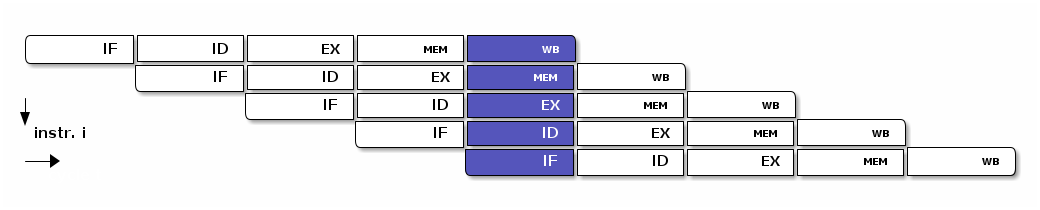
\includegraphics[width=1.0\textwidth]{figures/RISCPipeline.png}
\caption{\label{fig:PipelinedArchitecture}
Simple Pipelined Architecture}
\end{figure}


Simple pipelined architectures issue a single instruction per cycle.
Through pipeling, ILP is still exploitable, but limited by only having one of
each type of functional unit. Figure \ref{fig:PipelinedArchitecture} shows an
example simple RISC architecture with a 5 stage pipeline (IF=Fetch,
ID=Decode, EX=Execute,MEM=Memory Access,WB=Write Back) that exploits ILP while using only a single
execution unit. In contrast, figure \ref{fig:SuperScalarArchitecture} shows a
superscalar architecture that utilizes parallel execution units.  

\begin{figure}[htbp]
\centering
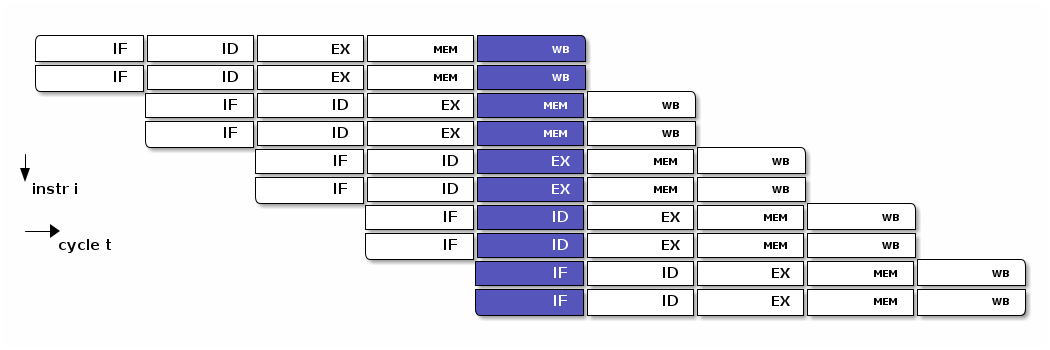
\includegraphics[width=1.0\textwidth]{figures/SuperScalarPipeline.png}
\caption{\label{fig:SuperScalarArchitecture}
SuperScalar Architecture}
\end{figure}


Superscalar architectures are all uniprocessors that can execute two or more
scalar operations in parallel; this encompasses a wide variety of
architectures, but common to all these architectures is the existence of
parallel and pipelined functional units, and the need to manage that
parallelism \parencite{zyuban2001inherently}. In particular, superscalar
architectures put increased strain on resource management. This poses a more
serious challenge for scheduling algorithms, since basic block scheduling is
often not sufficient to allow full utilization of machine
resources \parencite{bernstein1991global}. 

An simple architecture to schedule for would be a RISC architecture with
a collection of functional units of \(m\) types, where the machine has \(n_1\),
\(n_2\), \ldots{}, \(n_m\) units of each type. One could view optimizing a schedule over such
an architecture as maximizing the amount of live functional units per
cycle (i.e maximum throughput). This would generally be accomplished by
interleaving different types of instructions, however stretching data
dependent instructions too far apart doing runs the risk of running out 
available registers (increasing register pressure). 

\section{Pipeline Stalls}
\label{sec:orga3111e3}
Both of the previous figures \ref{fig:PipelinedArchitecture} and
\ref{fig:SuperScalarArchitecture} show an ideal schedule with \textbf{NO} stalls. A stall
occurs when, because of various architecture \textbf{hazards} that can arise, full throughput
cannot be achieved and a NOOP (No-Operation) instruction must be inserted.
This is also known as inserting a bubble in the pipeline.
Figure \ref{fig:PipelineStall} gives an example of inserting a NOOP (bubble),
because of a Read After Write (RAW) hazard.

\begin{figure}[htbp]
\centering
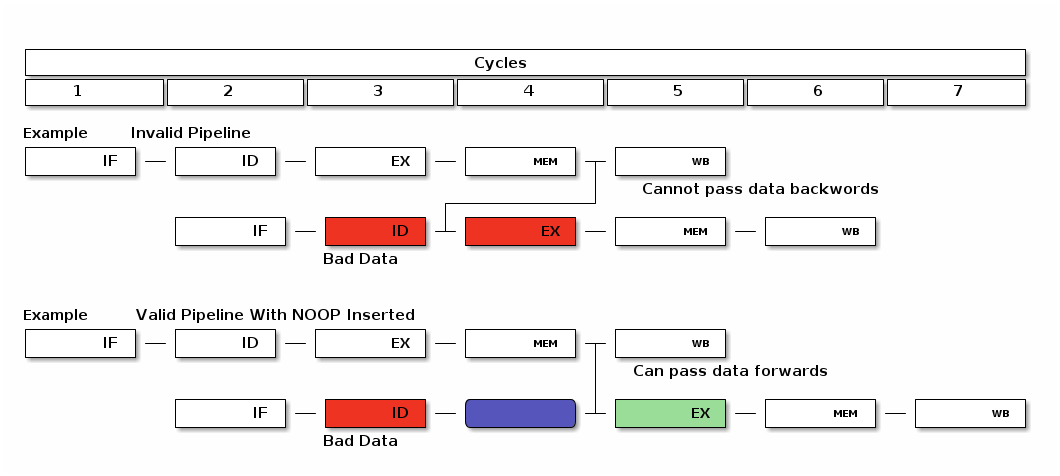
\includegraphics[width=1.0\textwidth]{figures/PipelineStall.png}
\caption{\label{fig:PipelineStall}
Example of a bubble (NOOP) being inserted to fix an unfullfilled data dependency}
\end{figure}

\section{Hazards}
\label{sec:org1649789}
Architecture hazards can be broken up broadly into three categories
\parencite{patterson2013computer}
\begin{itemize}
\item \textbf{Data Hazards} occur when a data dependency is broken. There are three
situations in which this can occur: read after write (RAW), write after
read (WAR) and write after write (WAW)
\end{itemize}
\begin{align*}
\textbf{RAW}                    & \qquad & \textbf{WAR}                   & \qquad & \textbf{WAW} \\
\textbf{R2} \leftarrow R5 + R3  & \qquad & R4 \leftarrow R1 + \textbf{R5} & \qquad & \textbf{R2} \leftarrow R4 + R7 \\
R4 \leftarrow \textbf{R2} + R3  & \qquad & \textbf{R5} \leftarrow R1 + R2 & \qquad & \textbf{R2} \leftarrow R1 + R3
\end{align*}
\begin{itemize}
\item \textbf{Structural Hazards} occurs when an aspect of hardware is accessed at the
same time (such as a functional unit)
\item \textbf{Control Hazards} also known as Branch Hazards, occur when a bad branch
prediction is made causing instructions that were brought into the
pipeline needing to be discarded
\end{itemize}
\section{Register Allocation via Graph Coloring}
\label{sec:orgd669639}
The theory of graph coloring deals with algorithms that seek to partition a
set of objects into classes, given simple rules associating objects that may
not belong to the same class \parencite{jensen2011graph}. These algorithms
operate on graphs, where the objects are vertices and the edges
denote connected vertices that cannot be in the same class. Classes are
represented via colors, where a \textbf{k-coloring} denotes a partitioning into k
distinct classes. The problem of finding a \textbf{k-coloring} is a well-known
NP-Complete problem \parencite{jensen2011graph}.

Architectures provide a finite set of registers that must be allocated
after or during instruction scheduling. Finding an allocation for a given
schedule (assuming one exists) has been shown to be equivalent to the Graph
Coloring problem and hence NP-Complete \parencite{chaitin1981register}. Given
a code schedule in Single Static Assignment (SSA) form, a unique interference
graph can be constructed that denotes data dependency. On an architecture
with \textbf{k} registers, a register allocation is found via a \textbf{k-coloring} of
vertices of this interference graph. See Figure \ref{fig:GraphColor} as an example.

\begin{figure}[htbp]
\centering
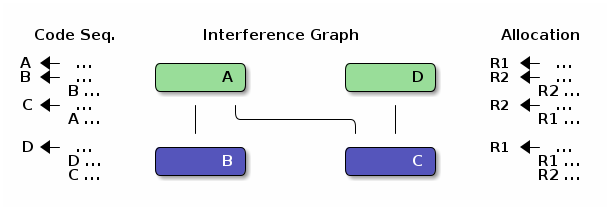
\includegraphics[width=.9\linewidth]{figures/GraphColor.png}
\caption{\label{fig:GraphColor}
Register Allocation via Graph Coloring}
\end{figure}

\section{Spilling}
\label{sec:org94e3182}
Finding the existence of a \textbf{k-coloring} for a given graph is itself an
NP-Complete problem \parencite{jensen2011graph}, and the absence of an
existing coloring presents a difficult problem. When a schedule cannot be
register allocated, variables must be \emph{spilled} to memory (spilling is the
action of storing variables into memory rather than registers
\parencite{bouchez2007complexity}). Spilling requires the addition of new
instructions to store/load from memory, which changes not only the
interference graph (allowing different register allocations) but the
dependency graph as well (allowing different schedules). Therefore adding spills
alters the space of valid schedules, and merits consideration when searching
for a "truly optimal" schedule (although addition of spills unnecessarily is
generally detrimental).

Graph coloring heuristics can be bolstered to include the addition of spilling
when they fail to find a proper \textbf{k-coloring}
\parencite{Chaitin:1982:RAS:872726.806984},\parencite{briggs1989coloring}. The
choice of which node to spill is a cost/benefit estimation. Each edge in the
interference graph can be assigned an estimated live range (sections of code
which a value is defined and used but not re-defined). Eliminating longer live
ranges alleviates more register pressure and creates a more flexible
scheduling space.

\section{Combining Register Allocation and Instruction Scheduling}
\label{sec:org6b88c17}
Register allocation can be performed before, after, or combined with
instruction scheduling, but is generally performed after
\parencite{brasier1995craig}. Performing allocation before scheduling
involves allocating on top of a "default" schedule and then manipulating the
schedule while maintaining a fixed allocation. Having a fixed allocation
creates new dependencies (known as \emph{anti-dependencies}) that limit the space
of valid schedules. Conversely, register allocation done after instruction
scheduling is uninhibited by these anti-dependencies and may find more
efficient schedules, but they may require post-hoc intervention via spilling.

Attempts to combine register allocation and scheduling are rare in
conventional compilers, as even a simple instance of the problem (single
register, no latencies, single functional unit) is \emph{NP-hard}
\parencite{motwani1995combining} \parencite{Pinter:1993:RAI:173262.155114}.
Heuristics developed for combining register allocation and scheduling
generally involve estimating a tradeoff between controlling register pressure
and instruction parallelism considerations \parencite{motwani1995combining}.

\section{Modulo Scheduling: Staging}
\label{sec:orge29af3f}
\begin{figure}[htbp]
\centering
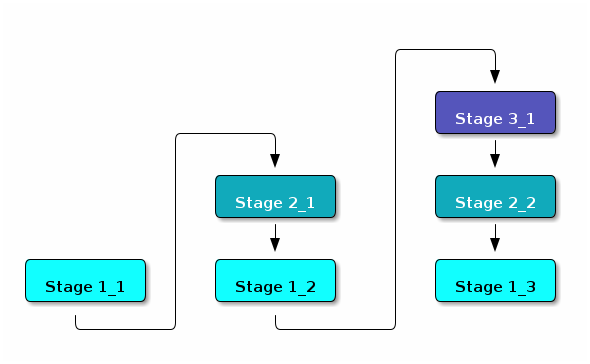
\includegraphics[width=0.6\textwidth]{figures/SwingModuloStaging.png}
\caption{\label{fig:SwingStaging}
Example 3-Staged for Modulo Scheduling}
\end{figure}

The objective of modulo scheduling is to engineer a schedule for one
iteration of the loop such that when this same schedule (known as the kernel)
is repeated at regular intervals, no intra- or inter-iteration dependence is
violated, and no resource usage conflicts arise between operations of either
the same or distinct iterations \parencite{rau1996iterative}. This generally
involves a sort of \emph{loop pipelining}, where a basic block of a loop can be
broken into stages and the loop can be \emph{unrolled} to interleave stages
between iterations (see Figure \ref{fig:SwingStaging}). Integral to this is the
concept of an \textbf{Initiation Interval} or II, which is essentially the fixed
delay between the start of successive iterations (see Figure
\ref{fig:InitiationInterval}). Each iteration of the loop can be divided into
stages each consisting of II cycles. A smaller II corresponds to shorter
execution time.

\begin{figure}[htbp]
\centering
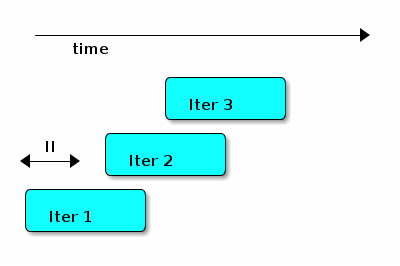
\includegraphics[width=0.6\textwidth]{figures/InitiationInterval.png}
\caption{\label{fig:InitiationInterval}
Initiation Interval}
\end{figure}

Modulo Scheduling algorithms require a candidate II be selected before
scheduling is attempted. The \textbf{Minimum Initiation Interval} or \(\operatorname{MII}\) is a lower
bound on the possible value of any II for which a modulo schedule exists. The
MII is constrained by both resource constraints (\(\operatorname{resMII}\)) and recurrence
constraints (\(\operatorname{recMII}\)). The resource constraint simply holds that resources
(such as functional units) must be sufficiently available and any extra
latency created waiting for a resource to become available must be accounted
for (the exact calculation of resMII is architecture specific and can
become very complicated on Out-of-Order execution architectures, covered in a
later section). The recurrence constraint lower bound is defined as the
maximum, taken over all cycles C in the dependence graph, of the sum of
latencies along C divided by the sum of distance along C:

\begin{align}
 \operatorname{MII} &= \max(\operatorname{recMII},\operatorname{resMII}) \\
 \operatorname{recMII} &= \max\limits_{C \in DepGraph} \frac{\sum\limits_{e \in C} latency(e)}{\sum\limits_{e \in C}
distance(e)} 
\end{align}
The task of generating an optimal, resource-constrained schedule for loops
with arbitrary recurrences is known to be NP-complete
\parencite{lam2012systolic}. A heuristic approach via Swing Modulo
Scheduling has been implemented in the GNU C Compiler (GCC)
\parencite{hagog2004swing}.

\section{Register Pressure In Staged Loops}
\label{sec:org3be2254}
Staging can increase throughput by enabling more instructions to
be scheduled between high latency operations and subsequent use.
However this also increases the number of live instances of loop
variables and thus requires more registers to accommodate the schedule.
Swing Modulo Scheduling (SMS) is a notable variation of modulo scheduling
that utilizes a heuristic approach that aims to reduce register pressure
\parencite{gosling2000java}. Some architectures also provide hardware
mechanisms for \textbf{Register Queuing} that provide more efficient spilling.

Due to the nature of modulo scheduling, the lifetime of a variable can
overlap with a previous definition of itself. To handle this, some form of
register renaming needs to be provided. Some hardware provides support for
this in the form of \textbf{Rotating Register Files} \parencite{rau1989cydra}. When
no hardware solution is provided, the problem of overlapping lifetimes can be
solved by a technique known as \textbf{Modulo Variable Expansion} (MVE), wherein the
kernel is unrolled and multiple definitions of a variable are renamed at
compile time \parencite{valluri1998modulo}. 

\section{Register Remapping/Renaming}
\label{sec:orgdd91334}
Not to be confused with renaming of registers at compile time, register
renaming in hardware is a technique to remove false data dependencies ---
write after read (WAR) and write after write (WAW) --- between register
operands of subsequent instructions at runtime \parencite{sima2000design}.
For example, a WAR hazard could be rewritten like so

\begin{align*}
\textbf{Before}                   & \qquad &                 \textbf{After} \\
R2 \leftarrow \textbf{R4} + R3    & \qquad &                 R2 \leftarrow \textbf{R4} + R3 \\
\textbf{R4} \leftarrow R1 + R5    & \qquad \Longrightarrow & \textbf{R33} \leftarrow R1 + R5
\end{align*}

A register renaming scheme must not rename to a register that would introduce
a new hazard, this would present a difficult problem were it not for the
existence of \textbf{Logical} and \textbf{Physical} Registers. When executing machine code,
hardware maps \textbf{Logical Registers} to \textbf{Physical Registers}
\begin{itemize}
\item \textbf{Logical Registers} are a set of registers usable directly when
writing/generating assembly code (limited by system architecture)
\item \textbf{Physical Registers} are a set of registers actually available in hardware
\end{itemize}
Having a larger number of Physical registers than Logical registers gives
hardware extra flexibility when dispatching instructions for \textbf{Out-of-Order Execution}.

\section{Out-of-Order Execution}
\label{sec:orge05b0b5}

The execution flow of an instruction on a CPU can be implemented in one of
two paradigms: \textbf{in-order} or \textbf{out-of-order} (OoO, also known as dynamic)
execution. Execution of an instruction cycle in each paradigm comprises
different steps:

\noindent
\textbf{In-Order Execution}
\begin{enumerate}
\item Instruction fetch
\item Stall until all operands are available
\item Dispatch to appropriate functional unit
\item Execute (on appropriate functional unit)
\item Write back to register file
\end{enumerate}

\noindent
\textbf{Out-Of-Order Execution}
\begin{enumerate}
\item Instruction fetch
\item Dispatch to a temporary queue known as \textbf{Reservation Station}
\item Wait in the reservation station until operands are available
\item Issue once operands are available (even if before an older
instruction)
\item Execute (on appropriate functional unit)
\item Retire results to another temporary queue
\item Write results back to register files after all older instructions have their results written back
\end{enumerate}

Although a more complicated design, OoO execution presents an opportunity to
increase throughput by filling in time that would be wasted stalling in step
2 of in-order execution with instructions that are ready, then re-ordering
the instructions back to appear they finished in order (known as retiring).
This essentially decouples the fetch and decode stages of the pipeline from
the execution stages. As the instruction pipeline deepens, there is therefore
increased opportunity to dispatch out of order. When combined with Register
Renaming, this is of particular benefit allowing instructions that are data
independent but register dependent to be executed in parallel. OoO
dispatching also provides benefits over in-order when cache misses (or high
latency memory accesses in general) occur \parencite{stark1997reducing}.
Figure \ref{fig:OutOfOrder} illustrates the general control flow in an OoO machine.

\begin{figure}[htbp]
\centering
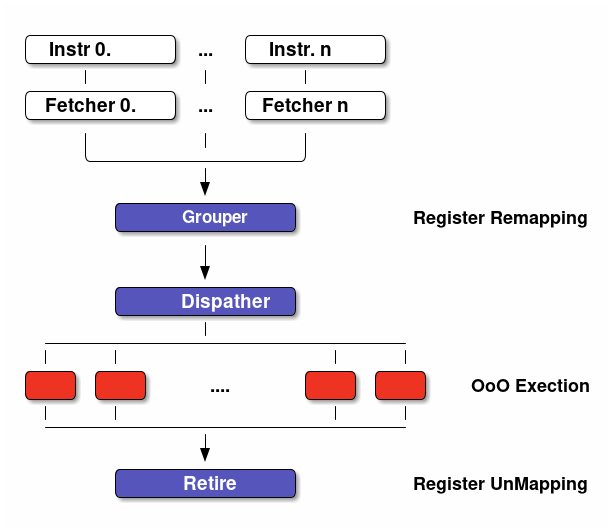
\includegraphics[width=0.7\textwidth]{figures/OoODiagram.png}
\caption{\label{fig:OutOfOrder}
Out-Of-Order Execution Control Flow}
\end{figure}

Out-of-Order execution requires dynamic scheduling (scheduling at runtime by
hardware) performed via methods such as \textbf{Tomasulo's Algorithm} or a \textbf{Register
Score-board}. Both methods seek to enable more efficient use of multiple
execution units while preventing breaking of data dependencies. A register
scoreboard checks resources for an instruction to see if the required
resources are available for the instruction to execute, and if so allows
dispatch. The scoreboard record (locks) the resources that would be modified
by the instruction at issue time, and any subsequent instructions that want to
access those resources cannot be issued until the instruction that initially
locked them subsequently unlocks them \parencite{popescu1997processor}.
Tomasulo's Algorithm innovated upon score-boarding by allowing improved parallel
execution although requiring new hardware features such as register renaming
in hardware, reservation stations for all execution units and a common data
bus between all reservation stations \parencite{tomasulo1967efficient}.

\chapter{Current State of the Art and Notable/Relevant Works in Instruction Scheduling}
\label{sec:org3dabd25}
\section{List Scheduling (most commonly performed scheduling)}
\label{sec:org6a8a2cb}
List scheduling is the most widely used technique for instruction scheduling
\parencite{gibbons1986efficient}. List scheduling encompasses a class of
algorithms for basic block scheduling via a chosen heuristic. It takes a list (of
instructions), assigns priorities via a heuristic and schedules them in a
topological order in decreasing priority \parencite{wang2018list}. The
general structure of a list scheduling algorithm can be described as follows

\def\mytitle{{\sc Basic Structure of List Scheduling Algorithms \hspace{12em} \color{grey}{.} }}
\begin{minted}[]{fortran}
while there are instrs to be scheduled do 
      Identify highest priority instr n
      Choose a processor p for n
      Schedule n on p at est(n,p)
end

est(n,p) = earliest start time of n on p
\end{minted}

Priorities can be static (remain constant for the DAG) or dynamic (change
through iteration of the algorithm). The complexity of list scheduling
depends on the heuristic, but is generally polynomial time
\parencite{wang2018list}. List scheduling can also be performed \emph{forward} or
\emph{backward}, or performed successively, applying heuristic on top of
heuristics. Examples of common heuristics are given in Table
\ref{tab:ListHeuristics} \parencite{sarangal2018list}.



\begin{table}[htbp]
\caption{\label{tab:ListHeuristics}
Example List Scheduling Heuristics}
\centering
\begin{tabular}{ll}
\textbf{Heuristic} & \textbf{Description}\\
\hline
HLFET & priority is chosen by the attributes\\
(Highest level first with estimate time) & of static levels\\
\hline
MCP (Modified Critical path) & priority by utilizing ALAP (As late\\
 & as possible) attribute\\
\hline
ETF (Earliest time first) & finds the earliest start time for each\\
 & task and later chooses the task having\\
 & less initial time\\
\hline
DLS (Dynamic level scheduling) & finds the task priority on the tasks\\
 & priority on dynamic basis\\
\hline
CNPT (Critical node parent tree) & prioritization of task is determined\\
 & with CN (Critical node) attribute\\
\hline
\end{tabular}
\end{table}


List scheduling is the chosen method for most conventional compilers because
of its flexibility, efficiency and ability to find near-optimal schedules for
most basic blocks. Although originally thought to yield near optimal
schedules for almost all schedules, analysis of list scheduling techniques
have shown that List Scheduling techniques have difficulty finding
near-optimal schedules for codes with a moderate amount of available
parallelism --- the peak difficulty varying with both the number of
processing elements and schedule length \parencite{cooper1998experimental}.
Therefore as architectures become more sophisticated and provide more
opportunity to exploit parallelism, list scheduling will in turn become
increasingly inadequate.

Limitations of list scheduling most likely stem from the use of a single
choice heuristic. There are many factors to consider when constructing a
schedule, and it is difficult (or more accurately impossible) to condense
this to assigning a priority via a polynomial time heuristic. As mentioned
before, combinations of heuristics can be applied through successive
iterations, but each iteration could undo previous iterations work.

\section{Constraint Programming}
\label{sec:org1575e98}
As an inherently discrete problem, a number of works have sought to formulate
instruction scheduling as an Integer Linear Programming (ILP) problem
(\parencite{wilken2000optimal}, \parencite{chang1997using},
\parencite{kastner2001ilp}, \parencite{nagarakatte2007register},
\parencite{kastner1999code}). These models optimize over integer objective
variables (representing schedule dispatch times for instructions), and
utilize constraints and penalties to achieve valid and desirable schedules.
Solving an ILP problem is an NP-Complete problem, so
formulating scheduling as an ILP only really serves to generalize
solutions to heuristics/approximation algorithms used by ILP solvers.

Another approach which has been far less investigated would be to optimize
the problem focusing entirely on constraints (known as constraint
programming). This type of optimization model would find a desirable schedule
through constraints alone (converting penalties). Notable efforts into this
approach are the works of McInnes/Beek in
\parencite{malik2008optimal},\parencite{van2001fast}. The constraint problem
in \parencite{malik2008optimal} found provably optimal schedules for basic
blocks , with the following types of constraints:
\begin{itemize}
\item \textbf{Latency Constraints}, i.e
\begin{itemize}
\item Given a labeled dependency DAG \(G = (N,E)\) 
\begin{itemize}
\item \(\forall (i,j) \in E \cdot j \geq i + l(i,j)\)
\end{itemize}
\end{itemize}
\item \textbf{Resource Constraints} that ensured functional units were not exceeded
\item \textbf{Distance Constraints}, i.e
\begin{itemize}
\item Given a labeled dependency \textbf{DAG}  \(G = (N,E)\) 
\begin{itemize}
\item \(\forall (i,j) \in E \cdot j \geq i + d(i,j)\)
\end{itemize}
\end{itemize}
\end{itemize}

The approach has some limitations on sophisticated enough architectures. The
hard constraints on latency would not account for \textbf{Register Remapping} in
\textbf{Out-Of-Order Execution} architectures that would be able to find more
optimal schedules despite the fact that latencies in normal execution would
create \textbf{pipeline stalls}.

\def\mytitle{{\sc Assembly Code Example Requiring Register Renaming for Optimal Scheduling \hspace{12em} \color{grey}{.} }}
\begin{minted}[]{haskell}
fma r3,r3,r4
fma r2,r2,r4
fma r4,r0,r3
fma r0,r1,r2
\end{minted}
On a system with only 5 registers and an instruction fma of large enough
latency, the scheduler would need to push these instructions apart to avoid
breaking the anti-dependency on register r4. However a machine
could use register remapping to execute these instructions efficiently Out-of-Order
making that constraint unnecessary. 

Despite limitations introduced by using hard constraints, this work is
notable as it illustrates how scheduling can be modeled as constraints. Even
with the limitations on OoO architectures cutting of the optimal schedule,
it's reasonable to assume the model would find near-optimal schedules. And by
converting hard constraints to soft constraints (penalties) its simple to
assert this space would contain the optimal solution.

\section{Stochastic Search}
\label{sec:orgc125d70}
There is a notable work to explore the space of schedules through a
stochastic algorithm by Schkufza, Sharma, Aiken at Stanford
\parencite{Schkufza:2016:SPO:2886013.2863701}. The efforts are culminated in
a piece of open source software known as STOKE that serves as a "stochastic
optimizer and program synthesizer" for x86-64 instruction sets. Stoke is a
super-optimizer with the following notable qualities:

\begin{itemize}
\item Suitable for \textbf{Short Basic Block} assembly code sequences (no modulo scheduling)
\item Utilizes a multi-pass algorithm, applying possibly overlapping program
transformations each pass
\item Encodes constraints as a \textbf{Cost Function} and uses a \textbf{Model Checker} to
ensure valid schedules (undo-ing transformations otherwise)
\item Uses \textbf{Markov Chain Monte Carlo Sampler} to add a stochastic element to
program transformation
\end{itemize}

Each pass of the optimization minimizes the cost function

\begin{equation*}
  \operatorname{cost}(R; T) = w_e \times \operatorname{eq}(R; T) + w_p \times \operatorname{perf}(R; T)
\end{equation*}

\begin{center}
\begin{tabular}{ll}
\(\color{lightgreen}{\boldsymbol{R}}\) & any rewrite of the program\\
\(\color{lightgreen}{\boldsymbol{T}}\) & the input program sequence\\
\(\color{lightgreen}{\operatorname{eq}(\cdot)}\) & the equivalence function (0 if \(\color{lightgreen}{R \equiv T}\) )\\
\(\color{lightgreen}{\operatorname{perf}(\cdot)}\) & a metric for performance\\
\(\color{lightgreen}{\boldsymbol{w_e}}\) & weight for the equivalence term\\
\(\color{lightgreen}{\boldsymbol{w_p}}\) & weight for the performance term\\
\end{tabular}
\end{center}

Limitations with the approach (as outlined in \parencite{Schkufza:2016:SPO:2886013.2863701}) include
\begin{itemize}
\item Only optimizes basic blocks (no loops)
\item Extremely innefficent (only practical for very short scheduling)
\item Cost function doesn't model the space of valid checking (hence model
checking is required per each rewrite)
\end{itemize}

This approach highlights the ability to use stochastic optimization to find
near-optimal schedules and the use of MCMC to explore the space of schedules.
Although the cost function doesn't model the space of valid schedules, using
it to generate schedules along with a model checker may still prove to be the
most practical way to explore a variety of schedules.

\section{Meta-Optimization / Hyper-Heuristics}
\label{sec:orgc7ed34e}
Meta-optimization deals with the use of one optimization method to tune
another one. 
Hyper-heuristics are an off-spring of meta-optimization, that search within the search space of heuristics vs. the entire problem solution space.
Hyper-heuristics are a relatively new concept (first used in 2000 to describe
heuristics to choose heuristics) the definition has more recently been
extended to refer to a search method or learning mechanism for selecting or
generating heuristics to solve computational search problems
\parencite{burke2013hyper}. When speaking of hyper-heuristics, two main
categories should be considered: heuristic \emph{selection} and heuristic
\emph{generation}. 

Previous research into meta-optimization of compilers has been attempted,
using machine learning to improve compiler heuristics
\parencite{stephenson2003meta}. The use of genetic programming has rarely
been used to solve production scheduling instances directly, because of the
difficulty of encoding solutions. However it has been found highly suitable
for encoding scheduling heuristics \parencite{jakobovic2007genetic}.

In the work of \parencite{jakobovic2007genetic}, genetic programming is used
to evolve dispatching rules, which are functions that assign a score to a job
based on the state of the problem. When a machine becomes idle, the
dispatching rule function is evaluated once for each job in the machine's
queue, and each result is assigned to the job as its score. The job in the
queue with the highest score is the next job to be assigned to the machine.
This approach shows genetic programming combining and rearranging heuristic
components to create heuristics superior to those which have been created by
humans (heuristic generation).

Although more works have investigated usage of heuristic generation for
scheduling (particularly through genetic programming
\parencite{beaty1991genetic},\parencite{kri2004genetic},\parencite{stephenson2003genetic},\parencite{wang2005instruction})
no works have been found (at the time of writing for this proposal) on
using heuristic selection / generation to analysis the effectiveness of
existing heuristics on scheduling in different architectures architectures.
Some work has been performed using ML in the form of Support-vector machines
(SVM) to learn compilation strategies (although not specific to scheduling)
in JiT compilers for the Java Virtual Machine \parencite{sanchez2011using}.

\chapter{Proposed Approaches To Stochastic Scheduling and Heuristic Analysis via Hyper-Heuristics}
\label{sec:org853782e}
In this section I will introduce a Stochastic Scheduling Algorithm that
utilizes a continuous optimization model with stochastically generated
parameters, and propose it's use as a training set generator for ML driven
heuristics selection and possibly generation. The full goal of this approach would
be to not only find a means to evaluate the effectiveness of scheduling heuristics on a
given architecture by observing learned heuristic selection, but to also be
able to evaluate the limitations of an architecture by analyzing the space of
valid schedules via the continuous model used for optimization.

\section{Optimization Model for Modulo Scheduling}
\label{sec:org664a85b}

The following is a specification for a continuous optimization model for instruction scheduling

\begin{align*}
    \color{lightblue}{\text{Objective Variables }} & t_i, b_i, f_i:& \mathbb{R} \\
    \color{lightblue}{\text{Indicator Function }} & \operatorname{IN} :& \mathbb{R} \rightarrow \mathbb{R} \\
    & t_i :& \text{dispatch time} \\
    & b_i :& \text{completion time} \\
    & f_i :& \text{FIFO use } 0 \leq f_i \leq 1 \\
     \color{lightblue}{\text{Constants }}& \operatorname{II} : & \text{iteration interval} = \frac{\# instructions}{dispatches/cycle} \\
\end{align*}

\begin{align}
    \color{lightblue}{\text{Hard Constraints }} \qquad & \forall i,j \cdot i \rightarrow j \qquad t_i + \epsilon \leq t_j  \\
								 & 0 \leq t_i \leq b_i \leq \#\text{stages} \cdot \operatorname{II}  \\
								 & b_i + \epsilon \leq t_i + \operatorname{II} \\
    \color{lightblue}{\text{Objective Function }} \qquad   & \text{min} \sum_{i} (b_i - t_i + f_i) + \text{Penalties}
\end{align}

The above is similar
to the work detailed in Constraint Programming by \parencite{malik2008optimal},
but only maintaining the constraints necessary for ensuring a valid schedule,
and relaxing the problem into a continuous domain as opposed to the Integer
Linear Programming models mentioned. This model contains a set of objective
variables: \(t_i\),\(b_i\),\(f_i\) for each instruction \(i\) to be scheduled. Each
variable \(t_i\),\(b_i\) represents the dispatch and completion times of the
\(i^{th}\) instruction respectively. As we wish to model an Out-of-Order execution
architecture, completion times are not necessarily fixed to dispatch times. The
third variable, \(f_i\), which is constrained to be between 0 and 1, is the
probability that the instruction \(i\) should spill. The constant variable
\(\operatorname{II}\) is the pre-computed Initiation Interval.

Unlike the work of \parencite{malik2008optimal}, the proposed model makes little
use of constraints. In fact the only constraints used are to enforce the
resulting schedule is a valid modulo schedule. The notation \(i \rightarrow j\)
used in the Hard Constraints equations above denotes that instruction \(j\)
depends on instruction \(i\). The first hard constraint enforces that any 
instruction must be dispatched only after it's dependencies. The second
constraint sets a limit on the overall execution time that instructions must
fall within. And the third constraint enforces that an instruction must complete
within the same interval it was dispatched to avoid an anti-dependency hazard. 

Without any \textbf{Penalties}, the above objective model would squash all dispatch and
completion times down, moving dependent instructions apart only by a given
\(\epsilon\) (a small constant) and assigning 0 to all \(f_i\). A \textbf{Key Idea} to this work: encode
choice heuristics as penalties, and adjust preference between heuristics by
scaling. Heuristics, such as the ones detailed for use in List Scheduling, can
all be encoded as Penalty Functions (functions that return a large value to push
down in the schedule, or a large negative value to push up). By picking a large
or small number to scale a penalty function we can prioritize a schedule.

\section{IO Penalty}
\label{sec:org1b57529}
Since we're not pushing instructions apart through latency constraints like
in \parencite{malik2008optimal}, we need a penalty to compensate. We propose
penalizing the dispatch time of instructions based on the quantity and
latencies of it's dependencies. \textbf{Note}: unlike a hard constraint on
latencies, this won't cut off valid schedules that could be optimal on OoO
architectures. 
\begin{align}
         \color{lightblue}{\text{Given }} \qquad  & t_i,t_j \qquad & \forall i,j \mid i \rightarrow j  \\
         \color{lightblue}{\text{For each i }} \qquad & N_j  =  \sum_{i \rightarrow j} \text{latency}(j) & \\
         \qquad & \qquad & \qquad \\
         \qquad & \mathbb{IO}(i) = \sum_{j} \frac{1}{N_j} \operatorname{IN}(t_i - t_j) & \qquad 
 \end{align}

\begin{figure}[htbp]
\centering
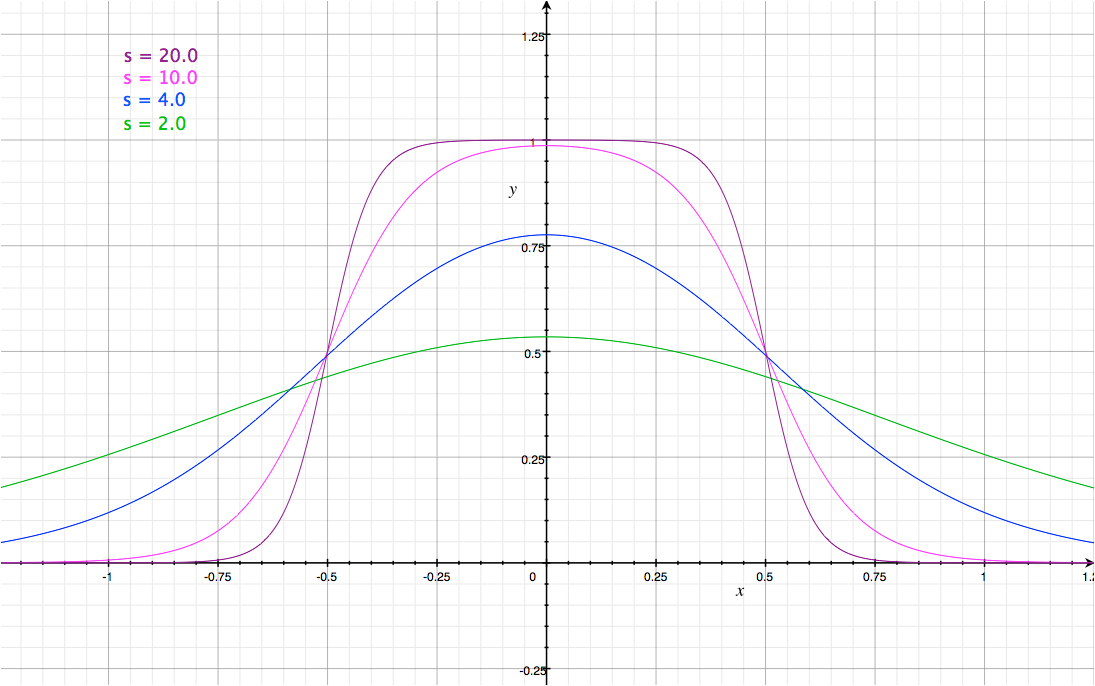
\includegraphics[width=.9\linewidth]{figures/sigmoid.jpg}
\caption{\label{fig:sigmoid}
Custom Indicator Function}
\end{figure} 

\section{Indicator Function}
\label{sec:org2380601}
The function \(\operatorname{IN}\) specified in the model and used in the IO Penalty
above is what's known as an Indicator Function, and is important for
implementing heuristics that rely on testing the proximity of two
instructions. Essentially, the function can be used to indicate (via a
non-zero value) whether two instructions are scheduled within a certain range
of each-other. For this purpose, we developed a custom indicator function (an
alteration of the sigmoid function often used in neural networks)
shown in Figure \ref{fig:sigmoid}.
\begin{align}
     S(x) = \frac{1}{(1 + e^{s(-0.5 + v)})(1 + e^{s(-0.5-v)})}
\end{align} 

\section{Stochastic Scaling}
\label{sec:orgef51b90}
The scaling \(\frac{1}{N_j}\) may be a good guess, but not necessarily effective in practice
\begin{itemize}
\item \textbf{IDEA} scale the \textbf{IO penalty} stochastically by a multiple of the II
\end{itemize}
\begin{align}
 \color{lightblue}{\text{Define a Grouping}} \qquad & \mathbb{C} = \text{Group}(\forall i \mid i \rightarrow j) \\
 \color{lightblue}{\text{For each Group i}} \qquad & c_i \in \mathbb{RAND(R)} \\
 \color{lightblue}{\text{Stochastic Penalty}} \qquad & \sum_i c_i II \cdot \mathbb{IO}(i)
\end{align}

As previously mentioned, various other heuristics can be encoded and also scaled
stochastically, in basically the same manner as the IO penalty. The nature
of many heuristics can be encapsulated by simply choosing the same scaling
based on the type of instruction (i.e push all loads up or down). 

\section{Opportunity for Hyper-Heuristic Development}
\label{sec:org363dff0}
By representing the space of schedules in a continuous model (i.e the space of
\(\mathbb{R}^n\)) and encoding heuristics as penalties, we can evaluate the
merits of various heuristics in combination with each other. The continuous
nature of the model provides more degrees of freedom when evaluating
overlapping heuristics. By scaling these heuristics stochastically, we
already have a method to analyze heuristic selection through analyzing which
scalings provide better performing schedules.

By generating a variety of schedules for different types of basic blocks using
the stochastic method we can also obtain a "training set" which can
subsequently be used with various supervised Machine Learning (ML) algorithms,
most notably Support Vector Machines (SVM), supervised learning models that
analyze data used for classification and regression analysis. The use of
neural nets, ensemble methods or genetic algorithms may also be worth
exploring.

Principal Component Analysis is a dimension reduction tool that can be used
to reduce a large set of variables to a small set that still contains most of
the information in the large set. Principal component analysis can possibly
be performed over the scaling parameters in conjunction with the training set
results in order to judge the influence of penalties on a given architecture.


Clustering methods (unsupervised learning) can possibly be used for heuristic
generation, by finding new groupings to scale. Given a clustering with scaling
\(c_i\) we can check the following assertion: For each scaling
\(\color{lightgreen}{c_i \in \mathbb{RAND(R)}}\), there exists an
\(\color{lightgreen}{\epsilon \in \mathbb(R)}\) such that
\(\color{lightgreen}{c_i + \epsilon}\) produces a distinct schedule from
\(\color{lightgreen}{c_i}\). If the assertion fails, the clustering is useless.
A prominent research question would be for this work would be whether or not
it's possible to avoid such clusterings. 

\chapter{Timeline}
\label{sec:orge7ec8e4}

\begin{table}[htbp]
\caption{\label{tab:ProposedTimeline}
Proposed Timeline}
\centering
\begin{tabular}{ll}
\textbf{Schedule} & \textbf{Goals}\\
\hline
\textbf{2020 Jan-Feb} & Write paper on stochastic scheduling\\
 & \\
\hline
\textbf{2020 Jan-Mar} & Update Coconut to schedule for POWER and release open-source\\
 & - \textbf{Jan} Simulator\\
 & - \textbf{Feb} CodeGraph Library\\
 & - \textbf{Mar} Update DSL\\
 & \\
\hline
\textbf{2020 May} & Present at IBM TechConnect\\
 & \\
\hline
\textbf{2020 Jun-Sept} & Generate Schedules for MASS on Power and experiment\\
 & with Hyper-Heuristic methods\\
 & \\
\hline
\textbf{2020 Jun-Aug} & Write paper on schedule optimization for OoO architectures\\
 & to submit to TACO\\
 & \\
\hline
\textbf{2020 Aug-Oct} & Write paper on Hyper-Heuristics to submit to one of the big\\
 & ML conferences (ICML,IJCAI,etc)\\
 & \\
\hline
\textbf{2020 Oct-Dec} & Attmpt to apply Hypr-Heuristic methods developed on power\\
 & to schedule for Z\\
 & \\
\hline
\textbf{2021 Jun} & Defend Thesis\\
 & \\
\hline
\end{tabular}
\end{table}

\addcontentsline{toc}{part}{References}
\printbibliography
\end{document}